\def\regenfigs{0}
\documentclass[anonymous,sigconf,9pt]{acmart}

\usepackage{microtype}
\if\regenfigs1
\usepackage{tikz,pgfplots}
\usetikzlibrary{arrows.meta}
\usepgfplotslibrary{groupplots}
\usepgfplotslibrary{external}
\usepgfplotslibrary{colorbrewer}
\pgfplotsset{cycle list/Set1}
\usepgfplotslibrary{fillbetween}
\pgfplotsset{compat=1.18}
\pgfplotsset{
    tick align=outside,
    tick pos=left,
    xmajorgrids,
    x grid style={white},
    ymajorgrids,
    y grid style={white},
    axis line style={white},
    axis background/.style={fill=white!89.803921568627459!black},
    legend style={draw=none, fill=none},
    legend cell align=left,
}
\pgfkeys{/pgf/number format/.cd, 1000 sep={\,}}

\pgfplotsset{
    log x ticks with fixed point/.style={
        xticklabel={
            \pgfkeys{/pgf/fpu=true}
            \pgfmathparse{2^\tick}%
            \pgfmathprintnumber[fixed relative, precision=4]{\pgfmathresult}
            \pgfkeys{/pgf/fpu=false}
        }
    },
    log10 x ticks with fixed point/.style={
        xticklabel={
            \pgfkeys{/pgf/fpu=true}
            \pgfmathparse{10^\tick}%
            \pgfmathprintnumber[fixed relative, precision=3]{\pgfmathresult}
            \pgfkeys{/pgf/fpu=false}
        }
    },
    log y ticks with fixed point/.style={
        yticklabel={
            \pgfkeys{/pgf/fpu=true}
            \pgfmathparse{2^\tick}%
            \pgfmathprintnumber[fixed relative, precision=4]{\pgfmathresult}
            \pgfkeys{/pgf/fpu=false}
        }
    }
}
\fi

\begin{document}

\begin{figure}[tbph]
\if\regenfigs1
\begin{tikzpicture}[overlay=false,>=latex]
    \begin{groupplot}[
            /tikz/overlay=false,
            /tikz/thick,
            group style={
                group size=1 by 2,
                vertical sep=0.7cm,
                xlabels at=edge bottom,
                ylabels at=edge left,
                %xticklabels at=edge bottom,
            },
            width=\linewidth,
            ylabel near ticks,
            xlabel={\# atoms},
            xmode=log,
            log basis x=10,
            %log10 x ticks with fixed point,
            clip=false,
            title style={yshift=-0.5cm, xshift=-2.8cm,anchor=west},
            ylabel style={xshift=1.6cm},
            height=2.1in,
        ]
            \nextgroupplot[
                %legend style={at={(0.0,0.6)},anchor=west},
                legend style={at={(1.0,0.3)},anchor=east},
                legend columns=3,
                title={a) Neighbor threading},
                transpose legend,
                ymode=log,
            ]
            \addlegendimage{empty legend};
            \addlegendentry{\hspace{-0.55cm}H100};
            \pgfplotsset{cycle list/Reds-5}
            \pgfplotsset{cycle list shift=3}
            \addplot+[mark=*]  table {results/pair/thread_h100_off.txt};
            \addlegendentry{off};
            \addplot+[mark=*]  table {results/pair/thread_h100_on.txt};
            \addlegendentry{on};
            \addlegendimage{empty legend};
            \addlegendentry{\hspace{-0.65cm}MI250X};
            \pgfplotsset{cycle list/Blues-5}
            \pgfplotsset{cycle list shift=0}
            \addplot+[mark=square*]  table {results/pair/thread_mi250x_off.txt};
            \addlegendentry{off};
            \addplot+[mark=square*]  table {results/pair/thread_mi250x_on.txt};
            \addlegendentry{on};
            
            \nextgroupplot[
                legend style={at={(0.0,0.6)},anchor=west},
                legend columns=4,
                title={b) Neighbor list style and Newton},
                transpose legend,
                ylabel={Speed [M\,atom-steps/s/node]},
            ]
            \addlegendimage{empty legend};
            \addlegendentry{\hspace{-0.55cm}H100};
            \pgfplotsset{cycle list/Reds-5}
            \pgfplotsset{cycle list shift=2}
            \addplot+[mark=*]  table {results/pair/neigh_h100_full.txt};
            \addlegendentry{full};
            \addplot+[mark=*]  table {results/pair/neigh_h100_half_off.txt};
            \addlegendentry{half, off};
            \addplot+[mark=*]  table {results/pair/neigh_h100_half_on.txt};
            \addlegendentry{half, on};
            
            \addlegendimage{empty legend};
            \addlegendentry{\hspace{-0.55cm}MI250X};
            \pgfplotsset{cycle list/Blues-5}
            \pgfplotsset{cycle list shift=-1}
            \addplot+[mark=square*]  table {results/pair/neigh_mi250x_full.txt};
            \addlegendentry{full};
            \addplot+[mark=square*]  table {results/pair/neigh_mi250x_half_off.txt};
            \addlegendentry{half, off};
            \addplot+[mark=square*]  table {results/pair/neigh_mi250x_half_on.txt};
            \addlegendentry{half, on};
    \end{groupplot}
\end{tikzpicture}
\else
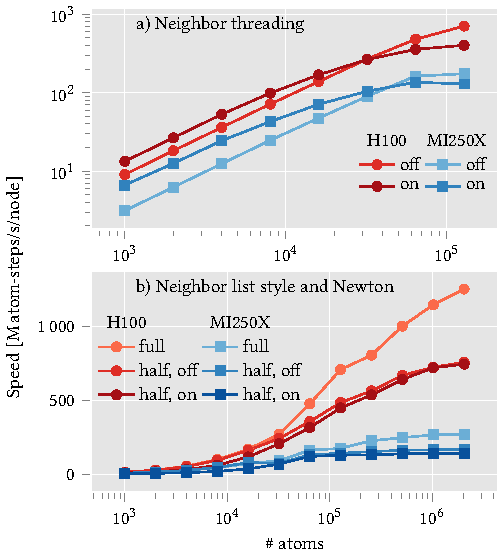
\includegraphics{generated-figures/paper-figure2.pdf}
\fi
% \vspace*{-10mm}
\caption{Performance effect of different options for a simple pairwise LJ potential. a) Effect of exposing parallelism over neighbors as a function of the number of atoms. For small systems, the benefit of additional parallelism outweighs the reduced efficiency of the more complex iteration pattern. b) Effect of redundant computations vs. thread-level atomic operations. With a full neighbor list, Newton's third law is ignored, and all pair interactions are computed twice. In return, this avoids the atomic operations and, with \texttt{newton on}, additional communication required with half neighbor lists. For simple pairwise potentials, whose computational cost is low, the full neighbor list is faster.}\label{fig:pair}
\end{figure}

\end{document}
